\section{Zielsetzung}
\label{sec:Zielsetzung}
Ziel des Versuches ist es verschiedene Formen periodischer Schwingungen
in ihr Frequenzspektrum zu zerlegen, beziehungsweise solche Formen
durch gezieltes überlagern verschieden frequenter Sinusschwingungen
zu erzeugen.

\section{Theorie}
\label{sec:Theorie}
Nach dem Fourieschem Theorem ist jede $T$ periodische Funktion
durch die Überlagerung einer $T$ periodischen Sinusschwingung
mit ihren Oberschwingungen in der Form
\begin{equation}
  f(t) = \frac{1}{2}b_0 + \sum_{n=1}^\infty a_n \text{sin}\left(n\frac{2\pi}{T}t\right)
  + b_n\text{cos}\left(n\frac{2\pi}{T}t\right)
  \label{eqn:sum}
\end{equation}
darstellbar. Für die Koeffizienten $a_n$ und $b_n$ gilt dabei folgendes:
\begin{equation}
  a_n = \int_0^Tf(t)\text{sin}\left(n\frac{2\pi}{T}t\right)d \, t
\end{equation}
\begin{equation}
  b_n = \int_0^Tf(t)\text{cos}\left(n\frac{2\pi}{T}t\right)d \, t
\end{equation}
Hierbei stellen die cosinus-Therme den symmetrischen und die sinus-Therme den
antisymmetrischen Anteil der Funktion dar. Ist eine Funtion also komplett symmetrisch
fallen alle sinus-Therme weg, sprich $a_n = 0$, ist sie antisymmetrisch gilt folglich
$b_n = 0$. Für den Versuch werden die folgenden antisymmertrischen Schwingungen verwendet.
\begin{figure}[H]
  \centering
  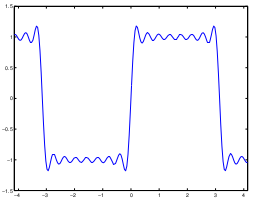
\includegraphics{content/images/rechteck_theo_n=15.png}
  \caption{Rechteckschwingung für die Partialsumme \eqref{eqn:sum} bis $n=15$\cite{koeff}.}
  \label{fig:rechteck_theo}
\end{figure}
Fourierkoeffizient zur Rechteckspannung
\begin{equation}
  a_n =
  \begin{cases}
      \frac{4}{\pi n} & \text{für ungerade } n\\
      0 & \text{für gerade } n
  \end{cases}
  \label{eqn:rechteck}
\end{equation}
\begin{figure}[H]
  \centering
  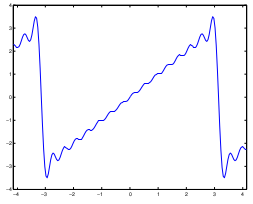
\includegraphics{content/images/saege_theo_n=15.png}
  \caption{Sägezahnschwingung für die Partialsumme \eqref{eqn:sum} bis $n=15$\cite{koeff}.}
  \label{fig:saege_theo}
\end{figure}
Fourierkoeffizient zur Sägezahnspannung
\begin{equation}
  a_n = (-1)^{n+1}\frac{2}{n}
  \label{eqn:saege}
\end{equation}
\begin{figure}[H]
  \centering
  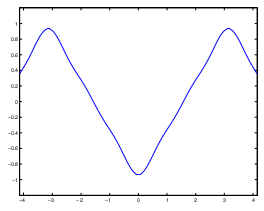
\includegraphics{content/images/dreieck_theo_n=5.png}
  \caption{Dreiecksschwingung für die Partialsumme \eqref{eqn:sum} bis $n=5$\cite{koeff}.}
  \label{fig:dreieck_theo}
\end{figure}
Fourierkoeffizienten zur Dreiecksspannung
\begin{equation}
  a_n =
  \begin{cases}
    \frac{-4}{\pi n^2} & \text{für ungerade }n\\
    0 & \text{für gerade }n
  \end{cases}
  \label{eqn:dreieck}
\end{equation}
Die Zerlegung einer bestehenden Schwingung in ihre Form als Fourierreihe
und das aufzeichnen des Frequenzspektrums wird Fourieranalyse genannt.
Die Fouriersynthese betitelt den Vorgang des gezielten Zusammensetzens
einer Spannungsform aus Grund- und Oberschwingungen durch die theoretischen
berechneten Fourierkoeffizienten.

\subsection{Prozentuale Abweichung}
Die prozentuale Abweichung berechnet sich nach
\begin{equation}
  \text{p} = 100\cdot \frac{a_\text{theo}-a_\text{exp}}{a_\text{theo}}.
\end{equation}
